\documentclass{article}
\usepackage[UTF8]{ctex}
\usepackage{amsmath,mathtools,geometry,pgfplots,float,mathrsfs,caption,enumerate}
\pgfplotsset{compat=1.15}
\usetikzlibrary{arrows}
\geometry{scale=0.7}

\newcommand\cusong[1]{
	\noindent \rlap{\hspace{0.01em}#1}\rlap{\hspace{0.02em}#1}\rlap{\hspace{0.03em}#1}\rlap{\hspace{0.04em}#1}\rlap{\hspace{0.05em}#1}#1
}


\title{\cusong{每日一题(21.2)}}
\author{\kaishu 李东宸}
\date{2022年6月15日}

\begin{document}
\maketitle
\begin{enumerate}
	\renewcommand{\labelenumi}{\textbf{\theenumi. }}
	\item 如图, 四边形$ABCD$为矩形, 面积为1234567890(这个数字可以为任何一个你喜欢的正实数). $F$为$BC$上的一点, $D$为$EG$中点, $AE\parallel FG$. 求梯形$AEGF$的面积.
	\begin{figure}[H]
		\flushright
		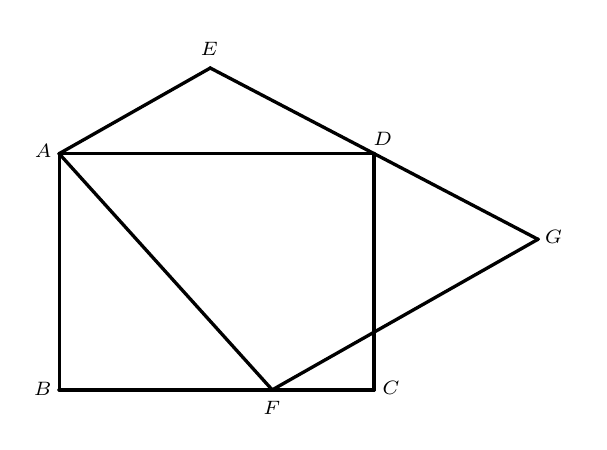
\begin{tikzpicture}[line cap=round,line join=round,>=triangle 45,x=1.0cm,y=1.0cm]
			\clip(-0.4,-0.4) rectangle (6.6,4.6);
			\draw [line width=1.2pt] (0.,3.)-- (0.,0.);
			\draw [line width=1.2pt] (0.,0.)-- (4.,0.);
			\draw [line width=1.2pt] (4.,0.)-- (4.,3.);
			\draw [line width=1.2pt] (4.,3.)-- (0.,3.);
			\draw [line width=1.2pt] (0.,3.)-- (2.705938816078333,0.);
			\draw [line width=1.2pt] (0.,3.)-- (1.9192235013179093,4.087571583313028);
			\draw [line width=1.2pt] (1.9192235013179093,4.087571583313028)-- (6.08077649868209,1.9124284166869723);
			\draw [line width=1.2pt] (2.705938816078333,0.)-- (6.08077649868209,1.9124284166869723);
			\begin{scriptsize}
				\draw [fill=black] (0.,3.) circle (0.5pt);
				\draw[color=black] (-0.2029124202923196,3.0340378053828205) node {$A$};
				\draw [fill=black] (0.,0.) circle (0.5pt);
				\draw[color=black] (-0.2104748697850276,0.016620457792352356) node {$B$};
				\draw [fill=black] (4.,0.) circle (0.5pt);
				\draw[color=black] (4.213558083449141,0.02418290728506029) node {$C$};
				\draw [fill=black] (4.,3.) circle (0.5pt);
				\draw[color=black] (4.107683790551229,3.1928492447296875) node {$D$};
				\draw [fill=black] (2.705938816078333,0.) circle (0.5pt);
				\draw[color=black] (2.7010681849075446,-0.23294037546700969) node {$F$};
				\draw [fill=black] (6.08077649868209,1.9124284166869723) circle (0.5pt);
				\draw[color=black] (6.278106794958419,1.9374826289401692) node {$G$};
				\draw [fill=black] (1.9192235013179093,4.087571583313028) circle (0.5pt);
				\draw[color=black] (1.9070109881732067,4.334779118128586) node {$E$};
			\end{scriptsize}
		\end{tikzpicture}
	\end{figure}
	\rightline{\tiny\kaishu (小学一年级趣味知识竞赛试题)}
	\item 如图, $P$为凸四边形$ABCD$中对角线$AC$和$BD$的交点, $M$为$AB$的中点, $MP$延长线交$CD$于$Q$. 证明:$\mathrm{S}_{\triangle BCP}/\mathrm{S}_{\triangle ADP}=CQ/DQ.$
	\begin{figure}[H]
		\flushright
		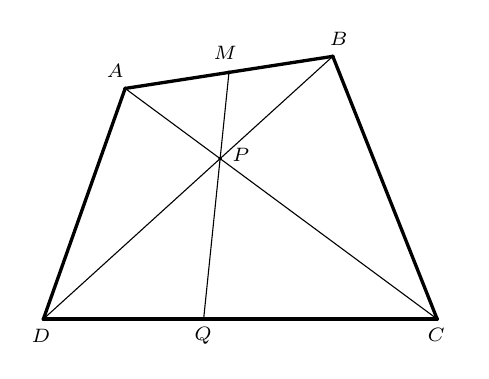
\begin{tikzpicture}[line cap=round,line join=round,>=triangle 45,x=1.0cm,y=1.0cm]
			\clip(-0.2,-0.4) rectangle (5.3,3.7);
			\draw [line width=1.2pt] (1.0380855414610588,2.9281635124849092)-- (3.6751116795683307,3.3357795401418673);
			\draw [line width=1.2pt] (3.6751116795683307,3.3357795401418673)-- (5.,0.);
			\draw [line width=1.2pt] (5.,0.)-- (0.,0.);
			\draw [line width=1.2pt] (0.,0.)-- (1.0380855414610588,2.9281635124849092);
			\draw [line width=0.4pt] (3.6751116795683307,3.3357795401418673)-- (0.,0.);
			\draw [line width=0.4pt] (5.,0.)-- (1.0380855414610588,2.9281635124849092);
			\draw [line width=0.4pt] (2.0347335202202634,0.)-- (2.3565986105146948,3.1319715263133885);
			\begin{scriptsize}
				\draw [fill=black] (1.0380855414610588,2.9281635124849092) circle (0.5pt);
				\draw[color=black] (0.9100056198781064,3.1530100341084637) node {$A$};
				\draw [fill=black] (3.6751116795683307,3.3357795401418673) circle (0.5pt);
				\draw[color=black] (3.751455588002711,3.55787984821948) node {$B$};
				\draw [fill=black] (5.,0.) circle (0.5pt);
				\draw[color=black] (4.988148838378187,-0.20372878833923413) node {$C$};
				\draw [fill=black] (0.,0.) circle (0.5pt);
				\draw[color=black] (-0.03223685659844641,-0.2110900576867072) node {$D$};
				\draw [fill=black] (2.3565986105146948,3.1319715263133885) circle (0.5pt);
				\draw[color=black] (2.3086467958979893,3.3812093838801274) node {$M$};
				\draw [fill=black] (2.244056366410047,2.0368570989589583) circle (0.5pt);
				\draw[color=black] (2.507401068279762,2.0782647093774025) node {$P$};
				\draw [fill=black] (2.0347335202202634,0.) circle (0.5pt);
				\draw[color=black] (2.0289185606940126,-0.2184513270341802) node {$Q$};
			\end{scriptsize}
		\end{tikzpicture}
	\end{figure}
	\rightline{\tiny\kaishu (小学一年级趣味知识竞赛试题)}
\end{enumerate}
\end{document}